\section{Spezialbefehle, Standardbefehle und Makros}

In diesem Kapitel werden einige Spezial- und Standardbefehle vorgestellt.
Eine vollständige Liste aller Befehle kann unter: \\ \textit{AddmusicK/readme\_files/syntax\_reference.html} eingesehen werden.

\subsection{Spezialbefehle}

Spezialbefehle erkennt man daran, dass sie mit einem \# beginnen (einizge Ausnahmen sind Kanalnummern). Alle Spezialbefehle müssen sich außerhalb der Kanäle befinden, einige müssen zwingend über den Kanälen oder in einer gewissen Reihenfolge platziert werden.


\subsubsection*{\#path \dq Pfadname\dq{}}

Falls Custom Samples verwendet werden sollen, gibt \#path den Pfad an, wo diese liegen (müssen sich in einem Unterverzeichnis von samples/ befinden).

\subsubsection*{\#samples\{\}}

Verwendete Custom Samples werden in \#samples\{\} gelistet. Neben den Samples muss sich zusätzlich eine Samplegroup bestimmt werden.

\medskip

\lstinputlisting[framexleftmargin=8mm, frame=shadowbox, rulesepcolor=\color{blue}, numbers=left, firstline=1, lastline=6]{codes/Spezial.txt}

\medskip

Anstelle von \#path kann auch der Pfad der Samples in den Namen angegeben werden.

\subsubsection*{\#samples\{\}}

In \#instruments\{\} können ADSR, Gain und Pitch eines SMW Samples, Custom Samples, oder Noise (Rauschen, wird benutzt um 8 Bit Percussions zu simulieren) definiert werden. Neu definierte Instrumente werden durchnummeriert, angefangen mit @30 und mit @ aufgerufen.

\medskip

\lstinputlisting[framexleftmargin=8mm, frame=shadowbox, rulesepcolor=\color{blue}, numbers=left, firstline=7, lastline=12]{codes/Spezial.txt}

\medskip

Für weitere Informationen zu \#samples\{\}, \#samplegroups und \#instruments\{\} siehe Kapitel \ref{sec:instrumente}.

\subsubsection*{\#spc}

Mit \#spc können Informationen zum Song hinterlegt werden, die in Lunar Magic und SPC Playern angezeigt werden.

\medskip

\lstinputlisting[framexleftmargin=8mm, frame=shadowbox, rulesepcolor=\color{blue}, numbers=left, firstline=13, lastline=20]{codes/Spezial.txt}

\medskip

Es können beliebig viele dieser Einträge benutzt werden.

\subsubsection*{\#halvetempo}

Halbiert das Tempo, Notenlängen und Hexbefehle, die eine Dauer verwenden. Nützlich, um Slowdowns zu umgehen, da diese maßgeblich durch zu hohes Tempo auftreten.

\subsubsection*{\#option}

Mit \#option, gefolgt von einem Schlüsselwort, können folgende Einstellungen vorgenommen werden:

\begin{table}[htbp]
	\begin{tabularx}{\textwidth}{|l|X|}
		\hline
		Parameter & Beschreibung\\
		\hline
		tempoimmunity & Das Tempo des Songs wird nicht erhöht, falls der SMW Timer unter 100 Sekunden ist.\\
		\hline
		dividetempo & Wie \#halvetempo, es kann aber ein anderer Divisor als 2 ausgewählt werden.\\
		\hline
		smwvtable & Der Song benutzt die SMW Lautstärketabelle anstatt der standard N-SPC Tabelle\\
		\hline
		noloop & Der Song wird nur ein einziges mal abgespielt und nicht geloopt.\\
		\hline
	\end{tabularx}
\end{table}

Beispiel: \#option dividetempo 3


\subsubsection*{\#define, \#undef, \#ifdef, \#ifndef, \#if, \#endif, \#error}

\subsection{Standardbefehle}

In diesem Kapitel werden Standardbefehle vorgestellt, auf einige davon wird näher eingegangen.
Eine vollständige Liste aller Standardbefehle befindet sich in der AddMusicK ReadME unter:
 \textit{AddmusicK\_1.0.8/readme\_files/syntax\_reference.html}
\bigskip


\subsubsection{Intros}

Ein Intro ist ein Bereich am Anfang eines Songs, der nur im ersten Durchgang durchlaufen wird. Alle Noten vor einem / werden einmalig gespielt. Sobald der Song endet, beginnt dieser hinter dem / zu spielen. \\
Es muss in jedem Kanal an der gleichen Stelle ein / stehen, damit die Kanäle synchron bleiben.

\subsubsection{Quantisierung}

Ein manchmal unterschätzter Befehl ist der Quantisierungsbefehl qXY, der gleich zwei Funktionen abdeckt. X und Y sind dabei Hexwerte, der Wertebereich von X liegt bei 0 - 7 und von Y bei 0 - F. \\
X \dq quantisiert\dq{} alle nachfolgenden Noten. Noten können dadurch um einen Faktor $ \dfrac{X}{8} $ verkürzt werden (Da wir bei 0 anfangen zu zählen, muss man gedanklich mit $X+1$ rechnen), die dadurch entstehenden zeitlichen Lücken werden automatisch mit entsprechend langen Pausen aufgefüllt. So entspricht ein q3F c4 einem c8 r8, was besonders hilfreich ist für Remote Codes, später dazu mehr. Außerdem belegt dieser Befehl keinen Speicher, normale Pausen allerdings schon. Dadurch lässt sich theoretisch weiterer Arbeitsspeicher einsparen.\\
Y ist ein Faktor um Lautstärken einzustellen. Dabei entspricht F einem Faktor von 1 und 0 einem Faktor von 0. In Kombination mit v und w lassen sich dadurch noch mehr Lautstärkewerte einstellen, was besonders hilfreich ist, falls man sehr genau andere SPC Dateien rekonstruieren will.

\subsubsection{Loops}

Wiederkehrende Notenabfolgen können in Loops zusammengefasst werden um Speicher einzusparen. Dabei unterscheidet man in zwei Arten von Loops: Loops und Superloops. Labeled Loops werden genau so wie einfache Loops behandelt da es auf technischer Sicht sich um die selbe Form von Loop handelt.


Ein Loop wird mit eckigen Klammern [ ] definiert, gefolgt von einer Zahl die angibt, wie oft der Inhalt wiederholt werden soll. Das Maximum beträgt hierbei 255. Beispiel:

\medskip

\lstinputlisting[framexleftmargin=8mm, frame=shadowbox, rulesepcolor=\color{blue}, numbers=left, firstline=1, lastline=1]{codes/Loop.txt}

\medskip

Ein sauberer Loop besteht immer aus gleich vielen > und <, dadurch ist die Oktave am Anfang und Ende des Loops identisch.

\bigskip

Ein bereits definierter Loop kann außerdem an anderer Stelle aufgerufen werden. Mit einem Asterisk \** wird der zuletzt verwendete Loop aufgerufen. Eleganter ist es allerdings, einen Loop über ein Label aufzurufen:

\medskip

\lstinputlisting[framexleftmargin=8mm, frame=shadowbox, rulesepcolor=\color{blue}, numbers=left, firstline=3, lastline=5]{codes/Loop.txt}

\medskip


Loops, die zu einem späteren Zeitpunkt nochmals aufgerufen werden bieten allerdings eine Fehlerquelle. Wird ein Loop definiert, wird die gerade verwendete Oktave für den Loop mit gespeichert.
Das nachfolgende Bild \ref{LabeledLoop} soll das Problem verdeutlichen.

\begin{figure}[htbp] \centering
	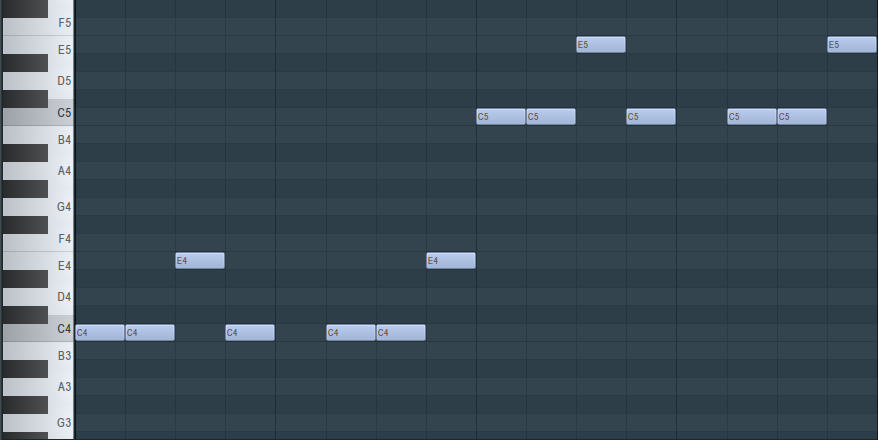
\includegraphics[width=.95\linewidth]{images/LabeledLoop1.png}
	\caption{Fehlerquelle Labeled Loop}
	\label{LabeledLoop}
\end{figure}

\medskip

\lstinputlisting[framexleftmargin=8mm, frame=shadowbox, rulesepcolor=\color{blue}, numbers=left, firstline=14, lastline=16]{codes/Loop.txt}

\medskip

Die intuitive Lösung wäre:

\medskip

\lstinputlisting[framexleftmargin=8mm, frame=shadowbox, rulesepcolor=\color{blue}, numbers=left, firstline=18, lastline=20]{codes/Loop.txt}

\medskip

Da die Oktave aber für den Loop selbst fest steht, würde beides mal die blaue Notenabfolge in Oktave 4 spielen. Das > beeinflusst den aufgerufenen Loop nicht, allerdings alle nachfolgenden Noten! \\
Korrekt ist folgender Ansatz:

\medskip

\lstinputlisting[framexleftmargin=8mm, frame=shadowbox, rulesepcolor=\color{blue}, numbers=left, firstline=22, lastline=25]{codes/Loop.txt}

\medskip

Mit

\medskip

\lstinputlisting[framexleftmargin=8mm, frame=shadowbox, rulesepcolor=\color{blue}, numbers=left, firstline=27, lastline=27]{codes/Loop.txt}

\medskip

werden alle nachfolgenden Noten um \$XX Halbtöne getuned und nicht die Oktave verändert.
\$0C sind 12 Halbtöne was genau eine Oktave entspricht.
Damit lassen sich auch Notenabfolgen Loopen, die sich nur durch eine konstante Halbtonschrittzahl unterscheiden! \\
Soll der Loop in die andere Richtung (also tiefere Noten) getuned werden, müssen von \$80 aus entsprechend viele Halbtöne abgezogen werden.

\bigskip

Mit Superloops kann man Loops verschachtelt. Sie werden mit doppelten eckigen Klammern [[ ]] definiert. Superloops können weder mit einem Label, noch einem Asterisk \** aufgerufen und kein weiteres mal verschachtelt werden. Beispiel:

\medskip

\lstinputlisting[framexleftmargin=8mm, frame=shadowbox, rulesepcolor=\color{blue}, numbers=left, firstline=7, lastline=12]{codes/Loop.txt}

\medskip

Das ursprüngliche Ziel, Speicher einzusparen kann allerdings auch verfehlt werden, denn das Definieren und Aufrufen von Loops kostet ebenso Speicher. \\
Einen Loop zu speichern benötigt 5 Bytes, 4 davon für den Loop selbst und 1 Byte für den Inhalt. Das aufrufen kostet dementsprechend jedes mal 4 Bytes.\\
Ein Superloop benötigt dagegen nur 4 Bytes, da ein Superloop nicht erneut aufgerufen werden kann und deshalb den Inhalt nicht abspeichern muss.

Im Vergleich dazu benötigt eine Note 2 Bytes bzw. 1 Byte, falls die vorherige Note die gleiche Länge besitzt. Daher muss man bei extrem kurzen Loops mit geringer Wiederholrate immer abwägen oder ggf. ausrechnen, ob sich ein Loop überhaupt lohnt.

\subsubsection{Makros}

Mit Makros können wir Schlüsselwörter erstellen die häufiger benutzt werden sollen. Definiert werden Makros außerhalb von Kanälen, die folgenden zwei Beispiele zeigen den Aufbau:

\medskip

\lstinputlisting[framexleftmargin=8mm, frame=shadowbox, rulesepcolor=\color{blue}, numbers=left, firstline=1, lastline=3]{codes/Standard.txt}

\medskip

Links vom Gleichheitszeichen steht der Variablenname mit dem der Inhalt auf der rechten Seite aufgerufen werden kann. Die Definition belegt keinen zusätzlichen Speicher.

\subsubsection{Remote Codes}